\documentclass{article}
\usepackage[utf8]{inputenc}
\usepackage{listings}
\usepackage{hyperref}
\usepackage{graphicx}
\usepackage{balance}
\usepackage{graphicx}
\usepackage{fancyhdr}
%\usepackage[margin=1.5in]{geometry}


\graphicspath{ {Images/} }
\DeclareGraphicsExtensions{.pdf,.png,.jpg}

\newcommand{\HRule}{\rule{\linewidth}{0.5mm}}


\begin{document}
\begin{titlepage}
\begin{center}

% Upper part of the page. The '~' is needed because \\
% only works if a paragraph has started.

\includegraphics[width=0.2\textwidth]{./logo}~\\[1cm]

\textsc{\LARGE University of Copenhagen}\\[1.5cm]

\textsc{\Large Language Processing II}\\[0.5cm]

% Title
\HRule \\[0.4cm]
{ \huge \bfseries Sentiment Analysis Of Multiclass Hotel Reviews \\[0.4cm] }

\HRule \\[1.5cm]

% Author and supervisor
\begin{minipage}{0.45\textwidth}
\begin{flushleft} \large
\emph{Author:}\\
Alexander \textsc{Wahl-Rasmussen} \\
Keith \textsc{Lia} \\
Maria \textsc{Barrett}
\end{flushleft}
\end{minipage}
\begin{minipage}{0.45\textwidth}
\begin{flushright} \large
\emph{KU Identity:} \\
\textsc{LGV740} \\
\textsc{DHL107} \\
\textsc{XXX123}
\end{flushright}
\end{minipage}

\vfill

% Bottom of the page
{\large \today}

\end{center}
\end{titlepage}
\pagestyle{fancy}
\lhead{}
\chead{\leftmark}
\rhead{}
\lfoot{Alexander, Keith \& Maria}
\cfoot{}
\rfoot{Page \thepage}

\tableofcontents
\vfill

\section{Introduction}

Sentiment classification is a sub-field of automatic text classification. According to \cite{pangetal} the majority of research in text classification has been on topic classification. User reviews are used extensively across the web. It is often related to e-commerce (products, services or shops) or more traditional review domains like books and movies. The vast majority are written from user-to-user. We have chosen to work with the hotel review domain. Booking a hotel stay is per se buying something you don’t know how turns out, because you buy a service before it’s provided. It is also a rather expensive experience and especially for vacations people put a lot of expectations into it. Therefore we believe that many people would put a lot of emphasis into other people’s experience with the hotel they consider booking - amongst this is user reviews. All big, online travel companies have large databases of user reviews. Furthermore people can express their opinion on other social media.  Sentiment classification can be useful for summarizing reviews across many different types of sites when ratings are absent or on different scales. 
\smallskip

In this assignment we report the method and results of classification sentiment in a 3-class task (negative, neutral, positive) on hotel reviews on a dataset we scraped from a travel company. We tried four different approaches: bag-of-words (BOW), valence shifters, wordlists and methods based on n-gram. We used two different measures: presence and TF-IDF. After we found that BOW performed best, we tried enhancing performance on this approach and found that boolean TF-IDF gave an accuracy of 0.9. 

\section{Constructing the dataset}
The dataset was scraped from orbitz.com. Orbitz.com is a travel company aimed primarily at North America and offering a wide range of travel services: \textit{flight ticket}, \textit{hotel}, \textit{car rental}, \textit{cruises} and \textit{vacation packages}. Hotel reviews have a salient position in the search overview, as seen in Figure \ref{fig:orbitz}. 

\begin{figure}[!ht]
	\centering
		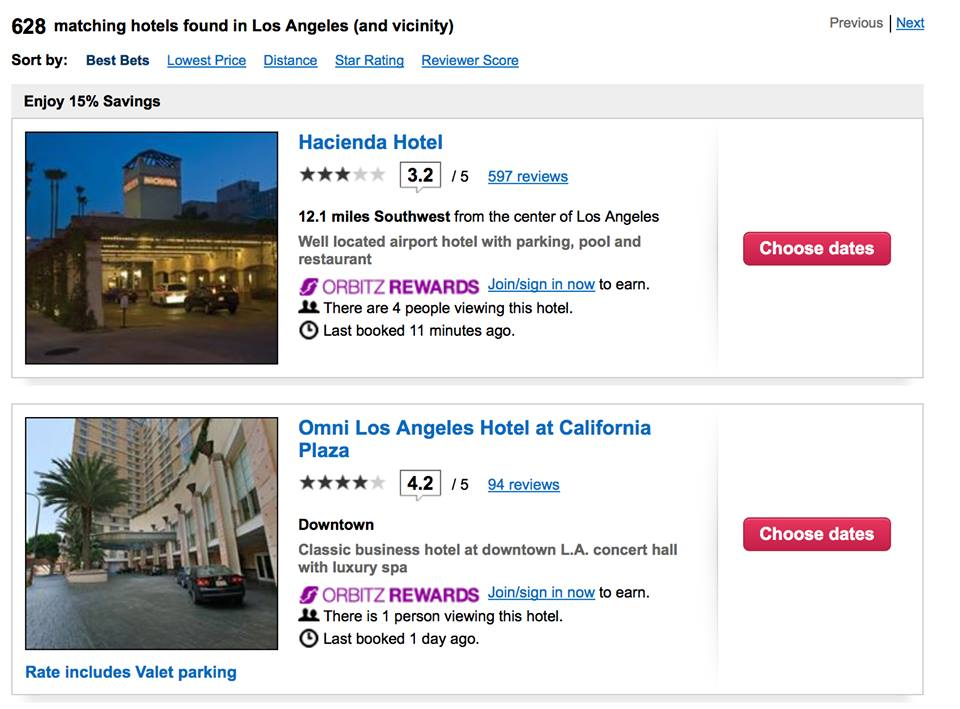
\includegraphics[height=8cm]{orbits}
	\caption{Screen dump of Orbitz.com}
	\label{fig:orbitz}
\end{figure}

We downloaded our review dataset by scraping the website, using this library: \url{http://www.cs.cornell.edu/~karthik/projects/hotelrev-scrape/}. There was a skewed distribution toward the positive reviews. We decided to over-sample and then balance the dataset because we would otherwise get a very large dataset or very few negative ratings. In this case, since we are using labelled data, oversampling is a common technique to try and reduce the bias between the classes as much as possible, and since we had the option to scrape more reviews, we decided to do so. 

We scraped all hotel reviews from the 10 largest cities in California which gave 24.329 reviews from 249 different hotels. They are stored in the file `\textit{ten\_cities\_reviews.csv}'. A review consist of a \textit{hotel name}, \textit{date} for the review, \textit{review text}, a \textit{rating} on a five-point Lickert scale and the \textit{hotel address} in a tab-separated format in a csv-file. For our purposes, we extracted only the review text and the five-point rating. 

\begin{table}[ht!]
  \centering
  \begin{tabular}{ p{25mm} | c | c | c | c | c |}
   
Rating & 1 & 2 & 3 & 4 & 5 \\ \hline\hline&&&&&\\
Count in over-sampled dataset & 1029  &1571& 4589& 11130& 6009\\
&&&&&\\Fraction in oversampled dataset&0.0422969& 0.064575&0.188630& 0.457497&0.246999\\
&&&&&\\Contribution to the balanced dataset&1000&&1000&&1000\\
\hline
  \end{tabular}
  \caption{Distribution of the review ratings}
  \label{tab:ratingstab}
\end{table}

Table \ref{tab:ratingstab} shows the distribution of the review ratings in our dataset. Positive rating is 5, Neutral rating is 3 and Negative rating is 1. By excluding rating 2 and 4 we presumably make the task easier by making the classes more separated. We constructed a balanced dataset consisted of 1000 positive, 1000 neutral and 1000 negative reviews. We took 1000 random draws from each pool of 1, 3 and 5 reviews. The random draws were seeded making our results reproducible. We then shuffled the balanced dataset which is also seeded. Like Pang et al. we did not use stemming or lemmatization. The dataset and the targets were stored using pickle in \textit{dataset\_easy.p} and \textit{targets\_easy.p}.

\section{On Python Libraries:  Sci-Kit Learn \& NLTK}
To extract the necessary features and correctly classify the reviews we utilized two Python libraries: Sci-Kit Learn\cite{web:sklearn} and NLTK\cite{web:nltk}. Both libraries are machine learning libraries, although NLTK has a focus on language processing where Sci-Kit Learn (SKLearn from now on) is a more general machine learning library. The reason why we chose to use both libraries is given by what we see as their difference in advantages and drawbacks.

The NLTK library is better than SKLearn at processing text. We used NLTK to sentence tokenize, word tokenize and to extract n-grams. SKLearn does support tokenizing and detecting n-grams, but documentation about this was poor, and we doubted that it would do it as good as NLTK. E.g NLTK can sentence tokenize and for word tokenization split contractions like `didn't' into two tokens: `did' and `n't'. 

NLTK also includes implementations of different algorithms, such as the Naive Bayes, but their documentation and variety of algorithms is somewhat lackluster. A small description of the principles behind the algorithm together with the source code is what is available for Naive Bayes \footnote{\url{http://www.nltk.org/_modules/nltk/classify/naivebayes.html} as opposed to \url{http://scikit-learn.org/stable/modules/naive_bayes.html} which includes theory, implementation examples, references and 3 different implementations}. As we were not satisfied with the documentation and the variety we instead chose to use SKLearn for the classifiers and NLTK to extract relevant features such as bigrams and trigrams. 

However, the issue of SKLearn is that it requires array-like input with integers and floats as the elements. Naturally, this can be overcome by converting the feature vectors into binary feature vectors, meaning the coding will be a bit more taxing than simply running NLTK out of the box. We see the benefit of proper documentation and variety as far outweighing in terms of results and robustness as opposed to using the out-of-the-box NLTK implementations. This is not to say that NLTK Naive Bayes' will perform worse than SKLearns\footnote{In fact, NLTK's Naive Bayes is run from SKLearn's}, but simply that we have more information on why SKLearn's implementations perform as they do.

\section{Method}
\subsection{Classifiers}
The chosen classifiers for our sentiment analysis are the Gaussian Naive Bayes and the Support Vector Machine with a radial kernel. As mentioned above, both classifiers are imported from the SKLearn library\cite{web:sklearn}.

As is evident from the choice of our classifiers, we presuppose that the dataset will fit nicely to a Gaussian distribution. We therefore presume that the distribution within each class is centered around the median with few outliers in an Euclidean space. It might not necessarily be the optimal distribution assumption when it comes to the actual fitting , but whether our assumption holds and allow us to reach sufficient results will be discussed in the later sections.

A \textit{ Support Vector Machine} tries to create a spatial decision boundary, where the shape of the decision boundary depends on the kernel. If a linear kernel is chosen the decision boundary is linear, and if the `rbf' kernel is chosen (as we did) the decision boundary becomes radial `clusters' that try to fit the data to a Gaussian. 
This resembles the approach of the Perceptron, but instead of trying to minimize the amount of errors, it creates the decision boundary at the maximum distance from the nearest support vectors. Intuitively this also means that the bigger the distance (or margin) is to the nearest support vectors, the lower amount of prediction errors should be on the seen data.
However, having a hard margin may result in overfitting the train set, which we can control with the hyperparameter C. Likewise we can control the smoothness of the Gaussian `clusters' with the hyperparamter $\gamma$. 

The \textit{Naive Bayes Classifier} is a simple probabilistic classifier that has the naive assumption of every parameter being independent. The classifier exists in many varieties which all rely on Bayes theorem. In its simplicity the theorem assumes that each feature independently contributes to the probability of a given input belonging to a certain class. This assumption naturally doesn't hold in the context of natural languages, but it has been shown to perform well despite its assumptional shortcomings\cite{pangetal}\cite{go}. 

As mentioned above, the SVM is a binary classifier meaning that it by default is only capable of classifying between two classes at a time. To overcome this constraint the SKLearn SVM has employed the OneVsOne-strategy where a classifier is trained per class pair.  Naive Bayes has no such constraint as it is inherently multiclass. With this in mind, we expect both classifiers to perform well in a multi-classification problem - but not necessarily with sentiment classification. 

Finally, to ensure good performance for both classifiers on all methods we trained the classifiers on our train set. With Naive Bayes it is as simple as calling its `.\textit{fit(x\_train,y\_label)}' function. As Naive Bayes has no hyper-parameters, it simply creates a lexicon of the probabilities of each label having specific features. With the radial SVM we had to do 5-fold cross-validation to ensure the optimal settings for the hyperparameters C and $\gamma$\footnote{with C ranging from 8 to 64, and $\gamma$ from 0.001 to 10}. We do not report on the specific hyperparameters as they change based on the feature input, but they are being printed when running the code. 

\subsection{Pre-processing}
In order to get the most out of the data and classifiers, we performed some pre-processing techniques which we will highlight in this section. 

Firstly, the dataset was imported into python from the pickle files as an array of reviews, and each review is in turn an array of sentences. 

We lower-cased the entire balanced dataset to get fewer different words. This may remove some information about sentiment, because you can express sentiment by use of capital letters ("I had NO complaints" vs "i had no complaints"), but most capital letters do not express sentiment, so we assume that lower-casing the corpus primarily removes noise and raises performance. It certainly reduces number of different tokens. 

We then loop through all the internal sentences and tokenize each one using the NLTK library. This helped us by splitting the words in the sentence into arrays, as well as extracting information such as punctuation marks, abbreviations and bound morphemes\footnote{An example of a bound morpheme which NLTK handles really well is in the case of `n't' in a word such as `didn't'}. 

We split our data into train and test set. Our train set consists of the first 2500, our test set of the last 500. 

In their paper, Pang et. al \cite{pangetal} experimented with both the presence of words as well as their frequency in the text, and therefore we decided to take the same approach in our implementation. To do the first one, we ran our dataset through a binarization algorithm. This looped through all of the reviews, looked at the words in our feature set, and marked them as 1 if they appeared in the review or 0 otherwise.  

The latter is approached in a similar manner, but instead of adding either a 1 or a 0, we count how many times the word appears in the review. If it never appears, a 0 is still added. The end result is the absolute frequency of the word in each review. To make the statistics even more informative, we performed the Term-Frequency/Inverse Document Frequency (TF-IDF) method using SKLearn's Feature Extraction function. TF-IDF compares the frequency of the words in the current review with the frequency of that same word in the train set. If it doesn't occur in many documents, it is given a higher weight. Vice versa, if it does occur a lot, then that means it is not as statistically significant if it is encountered in another document. This is a crude way of giving often used words in the entire train set (like function words and general hotel vocabulary) lower weight, but is no guarantee that words with a high TF are good features for sentiment classification. But the good features should probably be found among the words with a higher TF. SKLearn's function furthermore normalizes our data to zero mean unit variance which is the same as saying that it attempts to form a Gaussian distribution around 0. This is a good distribution to have when running it over the SVM with RBF kernel and a Gaussian Naive Bayes.

The approach described above result in two version of the feature vectors: a binarized feature vector and a feature vector with TF-IDF. The number of features vary with the method. There are more features in the n-gram based method than in BOW and there are more features in BOW than for the word list. 

\section{Methods}
\subsection{Lists of words expressing polarity or subjectivity}
An intuitive, but crude, method of trying to classify sentiment is to use a list of words expressing polarity or subjectivity as features - or word-list as we will refer to it from now on. This is also the baseline approach in \cite{pangetal}. 

The intuition behind the word-list method is quite simple: we use different words when we describe positive episodes as opposed to describing negative. This intuition seems reasonable as we have words exclusively describing positive and negative sentiments such as "good" and "bad". The next step is then to search every text for the appearance of these words and decide the sentiment based on the findings. If the only words we look for are "good" and "bad" then the decision is based solely on those and not anything else. 

\subsubsection{Our wordlist approach}
We first create 3 wordlists, where one list consists of positive words, one of negative words and the last a combined wordlist. The words can be found in Table \ref{tab:wordlist}. All of the words have been selected prior to inspecting the \textit{train} set, but with a check for words that did not appear in the train set at all. As is evident from the table below, we chose both "canonical" sentiment words such as a "good" and "bad", which has a more or less fixed sentiment, and more controversial words such as "cheap" and "old". However, we would argue that these controversial words are not that controversial considering the domain we are trying to classify. As mentioned in the previous sections, our domain consists of hotel reviews scraped from orbitz.com, meaning words that are seldom used to express sentiment in other domains, like conversations or film reviews, are frequent in a hotel review dataset.

Think of sentences such as "the hotel was cheap" or "the room was dirty and old" where the first sentence clearly portrays a positive attitude and the second a negative.
However, one could also argue that the opposite was true as e.g. "cheap" is often used negatively when describing a person, but we would argue that the positive interpretation is more frequent in this domain. 
Furthermore, we tried to balance the usage of domain-specific sentiments with more general sentiments as to not overfit completely.  

To classify the unseen reviews with our classifiers we first transform the combined wordlist to different feature vectors: one consisting of the binary representation of the word-list, effectively making it a small Bag-Of-Words\footnote{See the BOW section for a description of the BOW method}, and the other consisting of the TF-IDF score for each feature. 
For classification with our two different classifiers, we train the binary representation of the combined word list on the binary train set and test on the binary test set and repeat the procedure for the TF-IDF vectors. ALEX tjek lige om det er ok. Vi gentog bare for meget fra hvordan datasettet var lavet
The reason for using the combined wordlist is due to the fact that the classifiers themselves should learn from the training set what features are present in the positive class etc. The results can be seen table \ref{results} in the result section.


\begin{table}[ht!]
\centering
\begin{tabular}{ r | l }
 Positive words & Negative words \\
\hline \hline 
good & bad \\
wonderful & disgusting \\
perfect & terrible \\
best & wrong\\
love & worst\\
satisfied & awful\\
positive & ridiculous\\
amazing & hate\\
awesome & noisy\\
beautiful & negative\\
helpful & horrible\\
excellent & annoying\\
fantastic & small\\
great & uncomfortable\\
accommodating & waiting\\
cheap & rude\\
quality & wait\\
beautiful & dark\\
friendly & difficult\\
comfortable & bad\\
friendly & expensive\\
clean & dirty\\
close & stained\\
big & old\\
spacious & used\\
nice & smelly\\
\hline 
\end{tabular}
\caption{The positive and negative wordlists}
\label{tab:wordlist}
\end{table}

\subsubsection{Simple Classification}

The alternative, and the non-machine-learning approach, is to count the number of appearances of positive and negative words in each review. The decision on whether it is a positive, negative or neutral will then depend on the amount of positive and negative word in each document. If there are more positive words than negative it will be classified as positive, if reverse then negative and if equal then neutral.  

Our Simple Classification Algorithm:

\begin{lstlisting}
def simpleclassification(x_test,y_test,pos_words,neg_words):
    labels = []
    for doc in x_test:
   	 pos,neg = 0,0,
   	 for sent in doc:
   		 for i in xrange(len(pos_words)):
   			 if pos_words[i] in sent:
   				 pos +=1
   			 if neg_words[i] in sent:
   				 neg +=1
   	 if pos > neg:
   		 labels.append(2)
   	 elif neg > pos:
   		 labels.append(0)
   	 else:
   		 labels.append(1)
    score = 0
    for i in xrange(len(labels)):
   	 if labels[i] == y_test[i]:
   		 score +=1
    score = score/len(y_test)

    return score
\end{lstlisting}

The Simple Classification together with our baseline of labeling with the most frequent class taken in the train set\footnote{Which is subsequently the most numerous in the test set, but our classifier doesn't know that the dataset is balanced.}, are what the classifiers should outperform at the bare minimum before we can talk of having achieved a reasonable result.  

\subsection{Bag-of-Words}
The bag-of-words (BOW) model is a frequently used technique in natural language processing. It is used in order to represent text in numerical form, which machines can handle better, and is commonly used in document classification (alongside other techniques) where the appearance and frequency of a word can help determine what topic the document is talking about. In this context, the BOW model is used in conjunction with TF\_IDF.

However, while this works very well in classification tasks, sentiment analysis poses a more difficult problem. In topic classification, we can understand what the topic is about by extracting keywords in the text. In sentiment classification, the meaning is usually more abstract and one has to read 'in between the lines', which a machine is notoriously bad at. Despite the fact that the word '\textit{great}' appears in the text, the polarity of the sentiment can only be clear under context. Words like '\textit{not}' in front of it can change the meaning completely.

With this in mind, it is clear that the BOW model does not work as efficiently for sentiment analysis as it does with topic classification. However it has been shown by Pang et al. \cite{pangetal} that it still surpasses the baseline results, and thus it is worth while to investigate.

\subsubsection{Implementation}

The first step was to extract all the unique words from the dataset into a set. We keep track of all words which appear only once, and these are later removed, as part of the experiment discussed below. 

KEITH: Shouldn't it be: Words appearing only once in the train set were removed for the reduced feature set. Right now it sounds like they are removed for all conditions


Next, we traverse each individual review and convert the text into a counter object, containing each word and how many times it appears. Thus, the 'bag of words' is then constructed by looping through each review and extracting the words from each.

\begin{lstlisting}
for word in counter:
	if word in review:
		rep.append(review[word])
	else:
		rep.append(0)
\end{lstlisting}

In the above snippet of code, we loop through the whole set of unique words. If the word is found in the current review, we add the number of times it appears to the representation array '\textit{rep}'. If it never appears, a '0' is added to the array. As an example, the sentence '\textit{A boy and a dog}' would be converted into the following:

\begin{lstlisting}
{'a': 2, 'boy': 1, 'dog': 1, 'and': 1}
\end{lstlisting}

If our word set contains the following, as an example,
\begin{lstlisting}
{'a', 'boy', 'girl', 'dog', 'cat', 'but', 'and'}
\end{lstlisting}

our internal representation of the previous sentence would be an array of numbers, where the numbers are the amount of time the word appears in that particular review. The following is a representation of our example sentence.

\begin{lstlisting}
'A boy and a dog' - [2, 1, 0, 1, 0, 0, 1]
\end{lstlisting}

These absolute frequencies are then converted to relative frequencies using TF-IDF. By doing this, we transform the data into a Gaussian distribution, and in turn making it easier for the Gaussian SVM to handle. 

Another approach we took was that instead of taking the frequency into account, we look at whether the word appears in the review or not. This changes our internal representation from relative frequencies to a binary `yes/no'. Therefore, our previous example would differ by only having 1's and 0's, as follows:

\begin{lstlisting}
'A boy and a dog' - [1, 1, 0, 1, 0, 0, 1]
\end{lstlisting}

\subsubsection{Results}
Pang et al. \cite{pangetal} achieved their best results with a Naive Bayes classifier when using word frequency, and SVM when using word presence on their unigram benchmark. We have decided to replicate their experiments using both classifiers to see whether our data set produces similar accuracies. The SVM ran through a 5-fold cross validation, and used a grid search algorithm in order to find the best hyper-parameters C and $\gamma$. 

We split the tasks using `\textit{frequency vs. presence}' and `\textit{all vs. reduced features}'. Therefore, each classifier was run four times with the different parameters, as is shown in Table \ref{tab:bowresults}. The number of features were changed to check whether having a smaller, more concise set would reduce the noise and thus increase the accuracy, especially for SVM. Our whole training data set consists of 9.874 features, whereas the reduced data set, which was created by removing all the words that appeared only once, has 4.607 features.

\begin{table}[ht!]
  \centering
  \begin{tabular}{ r | c | c | c }
    Classifier & no. of feats & freq/pres & Accuracy \\
		\hline \hline
		Naive Bayes & All & freq & 87.4\% \\
		& All & pres & 88.2\% \\
		& Reduced & freq & 84.2\%\\
		& Reduced & pres & 89.2\%\\
		\hline
		SVM & All & freq & 87.6\%\\
		& All & pres & 78.0\% \\
		& Reduced & freq & 89.2\% \\
		& Reduced & pres & 77.8\% \\
		\hline
  \end{tabular}
  \caption{Results on BOW model of two classifiers using frequency vs presence of words}
  \label{tab:bowresults}
\end{table}

In our initial results, Naive Bayes performs better on word presence, giving the best score at 85\% with the reduced dataset. The SVM worked better with term frequency, and gave the highest overall accuracy overall of 85.4\% with the entire dataset. 

We then ran some further tests to improve on the results by combining the presence of the word with the inverse document frequency. This is called `binary frequency', and is similar to TF\_IDF. However, in this case, the weighting will be calculated on how many documents the word appears in. Therefore, if the term appears in fewer documents, it will get a higher weighting. This technique gave us very good results on the SVM, as reported in Table \ref{tab:bowresults2}. On the contrary, it diminished the accuracies for the Naive Bayes, so for the sake of clarity we chose not to report them.

\begin{table}[ht!]
  \centering
  \begin{tabular}{ r | c | c | c }
    Classifier & no. of feats & freq/pres & Accuracy \\
	\hline \hline
		SVM & All & pres & 90.4\% \\
		& Reduced & pres & 89.8\% \\
		\hline
  \end{tabular}
  \caption{Results on SVM using IDF on word presence}
  \label{tab:bowresults2}
\end{table}

\subsubsection{Discussion}
Like Pang et. al \cite{pangetal}, both classifiers worked best with word frequency, and Naive Bayes outperformed SVM on word presence alone. Using binary frequency also boosted the SVM's performance drastically, suggesting that the inverse document frequency is a very informative feature not just when doing topic classification. 

From Table \ref{tab:bowresults}, we can see that reducing the number of features helps the Naive Bayes classifier. Our motivation behind this was that by doing so, we reduce any noisy data. Of course, one could argue that by removing words, we're potentially cutting off possible informative features, and this is more true for when we look at the TF-IDF method, since lower appearing words will have more weight. However, if a word appears only once throughout the entire training set, the chances of it appearing again are very slim. Furthermore, feature selection has been shown to give better results by reducing over-fitting. 


\subsection{Methods based on n-grams}
N-grams is similar to BOW, but instead of tokens, n-grams are n succeeding tokens. We report results from bigram and trigrams. Below is an example of bigrams and trigrams from a made-up sentence:\textit{sentence = [`this', `is', `the', `best', `hotel', `ever', `!']}. \textit{bigrams = [(`this', `is'), (`is', `the'), (`the', `best'),(`best, `hotel'), (`hotel','ever'),(`ever','!')]} \textit{trigrams = [(`this','is','the'),(`is','the','best'), (`the','best','hotel'), (`best','hotel','ever'), (`hotel','ever','!)].}

The longer the n-grams, the more different n-grams and the lower the overall frequencies. Longer n-grams has the advantage of encompassing more context, but if the dataset is small or the authors use different words or word combinations, then the frequency of each n-gram will be too low to be significant. Hence it depends on the dataset which n is the best for a specific dataset. The n-grams must be extracted per sentence so you don't get the trigram \textit{(`more', '.', 'we')} out of these two sentence: \textit{[... [`i', 'could', 'n't', 'take', 'more', '.'] , ['we', 'left', 'early']...]}. Like for the other tasks we both counted presence (binary vectors) and TF-IDF (float vectors). 

\subsubsection{Making n-grams}
The biggest challenge when performing n-gram classification is dealing with a lot of features. 
We used all the n-grams found in the train set as gross feature set. This is different from the approach in the NLTK book Chapter 6.1 in the section “Document Classification” (example code 6.5), where the feature set was constructed from all features from the entire data set (both train and test set) - though they did bag-of-words instead of n-grams. The test set should not be used for building the model, but should be kept unseen for the model until the moment of testing. We find it more appropriate only to use the train set n-grams, because the approach described in the book leads to overfitting. Though we may have gotten a better accuracy from following the book, we would not get a measure of our model’s ability to generalize to un-seen data, which is the whole idea of building a model. 

We extracted 67.052 different bigrams and 127.175 different trigrams from the sentences in train set using the NLTK library. They constitute the gross feature sets from which the good features should be found. The very most frequent n-grams are not suitable for sentiment classification, because they are common for the 3 classes. E.g. the 5 most frequent bigrams are: \textit{('the', 'hotel'), ('in', 'the'), ('the', 'room'), ('it', 'was'),('of', 'the')}. Not surprisingly they contain function words and then a few words revealing something about the topic. So we don’t want just the very most frequent n-grams, but we don’t want all 67.0.52 / 127.175 either. Especially SVM is prone to the curse of dimensionality because it uses distances between data points and the decision boundary. This means that if there are too many features, the effect of the important features will ‘wash out’ in the noise from all other features. Naive Bayes does not have this limitation but will also benefit from a bit of help to avoid a lot of features not to mention that having this amount of features is computationally very expensive.

\subsubsection{Feature selection using decision tree}
To do feature selection we used a random forest of 100 CART decision trees\footnote{\url{http://scikit-learn.org/stable/modules/generated/sklearn.ensemble.ExtraTreesClassifier.html}}. A decision tree can also be used for classification and regression and it works by finding the features that gives the highest information gain (equal to the smallest entropy) to split by and therefore it can also be used for feature selection i.e the most important feature is the feature giving the largest information gain. 

Decision trees work roughly by calculating the entropy for all features in a train set. It selects the feature giving the smallest entropy to split by and creates a decision node. 
Then it repeats for the remaining features and datapoints until there are no more features or no more datapoint datapoint or all remaining datapoints are of the same class. The last node on a branch is a leaf specifying a class label. After a long training the is ready to give you the important features or predict very fast. You can set some pruning parameters e.g. minimum leaf size, max depth that prevents overfitting. 

Decision trees works with more than two classes without any modifications. It does tend to overfit however, which is why we use a random forest instead of a single tree. The random forest returns a list of features sorted by importance, and we also plotted the result. The plots can be seen below / in appendix. We used visual inspection (similar to scree test) of the sorted feature importances to decide how many features we wanted. We decided on 1000 and used CART to return the indices for the 1000 most important features. The remaining features were discarded and we performed SVM and Naive Bayes only using this subset. We performed feature selection on bigram, trigram for both the binary and TF-IDF. Below can be seen the 20 most important features for bigram and trigram for the binary task  along with its importance value. 
\vfill

\textbf{BIGRAM binary}\\
1. feature, name: ('a', 'great'), importance: 0.007306\\
2. feature, name: ('was', 'not'), importance: 0.006044\\
3. feature, name: ('had', 'to'), importance: 0.005949\\
4. feature, name: (',', 'but'), importance: 0.005222\\
5. feature, name: ('clean', 'and'), importance: 0.004832\\
6. feature, name: ('very', 'clean'), importance: 0.004463\\
7. feature, name: ('did', 'not'), importance: 0.004349\\
8. feature, name: ('will', 'never'), importance: 0.004213\\
9. feature, name: ('was', 'great'), importance: 0.004024\\
10. feature, name: ('do', "n't"), importance: 0.003742\\
11. feature, name: ('the', 'worst'), importance: 0.003654\\
12. feature, name: ('this', 'hotel'), importance: 0.003621\\
13. feature, name: ('i', 'was'), importance: 0.003337\\
14. feature, name: ('but', 'the'), importance: 0.003258\\
15. feature, name: ('on', 'the'), importance: 0.003206\\
16. feature, name: ('do', 'not'), importance: 0.003161\\
17. feature, name: ('in', 'the'), importance: 0.003133\\
18. feature, name: ('very', 'nice'), importance: 0.003115\\
19. feature, name: ('the', 'hotel'), importance: 0.003093\\
20. feature, name: ('a', 'little'), importance: 0.003077
\\

\textbf{TRIGRAM binary}\\
1. feature, name: ('i', 'will', 'never'), importance: 0.004819\\
2. feature, name: ('[', '...', ']'), importance: 0.003773\\
3. feature, name: ('did', "n't", 'work'), importance: 0.003764\\
4. feature, name: ('will', 'never', 'stay'), importance: 0.003159\\
5. feature, name: ('very', 'clean', 'and'), importance: 0.002924\\
6. feature, name: ('room', 'was', 'not'), importance: 0.002831\\
7. feature, name: ('the', 'front', 'desk'), importance: 0.002679\\
8. feature, name: ('not', 'worth', 'the'), importance: 0.002628\\
9. feature, name: ('was', 'great', '.'), importance: 0.002531\\
10. feature, name: ('was', 'a', 'great'), importance: 0.002358\\
11. feature, name: ('in', 'the', 'room'), importance: 0.002287\\
12. feature, name: ('would', 'not', 'recommend'), importance: 0.002179\\
13. feature, name: ('i', 'had', 'to'), importance: 0.002157\\
14. feature, name: ('for', 'the', 'price'), importance: 0.002085\\
15. feature, name: ('on', 'the', 'floor'), importance: 0.002079\\
16. feature, name: ('the', 'rooms', 'are'), importance: 0.001920\\
17. feature, name: ('within', 'walking', 'distance'), importance: 0.001908\\
18. feature, name: ('i', 'would', 'not'), importance: 0.001894\\
19. feature, name: ('the', 'hotel', 'was'), importance: 0.001853\\
20. feature, name: ("n't", 'stay', 'here'), importance: 0.001846 \\
\newpage

Besides general n-grams expressing content or discontent like ('will', 'never', 'stay'),('was', 'a', 'great') or ('the', 'worst') then you can say, that what separates a positive, neutral and negative hotel experience was e.g. whether or not the something concerning the front desk was described, whether something was within walking distance, cleanliness or something wasn’t working. ‘but’ is present in two important n-grams, which can be due to the fact that we included a neutral category. In a neutral category some things are good, but others aren’t. 

\subsection{Polarity and intensity shifters}

\subsubsection{Valence shifters}
\cite{pangetal} and \cite{kennedy} use valence shifters. \cite{polanyi} describes different contextual valence shifters including negations, which they call sentence-based valence shifters. They use more shifter words than Pang et al, who only report using ‘n’t’ as shifters. \cite{polanyi} suggest the following words as negative valence shifters: 'n’t’, ‘not’, ‘never’, ‘none’, ‘nobody’, ‘nowhere’, ‘nothing’, ‘neither’ by arguing that the valence for the rest of the sentence has shifted e.g. for a sentence like “John is never successful at tennis”. We used the negative words suggested by \cite{polanyi}. \cite{pangetal} did not report a great benefit from this approach and \cite{kennedy} suggest it may be of most impact for a simple count of positive and negative words. Therefore we only report results of valence shifters on wordlist. 

We implemented it like this: On the tokenized dataset we searched for the word above. If we encountered a word, the rest of the sentence had a ‘NOT\_’ added to the beginning of the word. This led to sentences like below, where the NOT\_ seem to add the appropriate valence e.g. to ‘offer’ and ‘help’, which are positive words in a hotel review. It also creates a lot of extra tokens, which may add noise to the dataset. 

['he', 'did', "n't", 'NOT\_offer', 'NOT\_any', 'NOT\_way', 'NOT\_to', 'NOT\_help', 'NOT\_-', 'NOT\_folding', 'NOT\_cots', 'NOT\_,', 'NOT\_anything', 'NOT\_.']

\section{Results}
\begin{table}[ht!]
  \centering
  \begin{tabular}{ | r | p{10mm} | p{10mm} | p{10mm} | p{10mm} | p{10mm} | p{10mm} | p{10mm} | p{10mm} | }
Classifiers & BOW & Bigram presence & Bigram & Trigram presence & Trigram & Word-lists & Valence word-lists
& BOW polarity \\
\hline \hline
Baseline&0.298&0.298&0.298&0.298&0.298&0.298&0.298&0.298\\
\hline
Simple Classification&&&&& 0.554 &0.554\footnote{Simple Classification does not run with TF-IDF score, but with absolute frequency instead.} &&\\
\hline
Naive Bayes& &0.588&0.638&0.546&0.576&0.51&0.486&\\
\hline
SVM&&0.68&0.678&0.572&0.598&0.622&0.608&\\
\hline
  \end{tabular}
  \caption{Accuracies from all methods and both classifiers. Best performance of each method in bold. }
  \label{tab:resultsfinal}
\end{table}



All the results are with the TF-IDF feature vectors unless otherwise specified. We chose to only report the results from the TF-IDF feature vectors as they generally had a higher accuracy and to increase the clarity of the table.

\section{Discussion}

\subsection{Why is the initial distribution skewed?}
In the initial distribution the two negative ratings only contributed about 10 \% of all reviews. To us it makes little sense that there are so few negative reviews. Our initial assumption was that hotel quality would be perceived from the customers as a gaussian distribution: most middling experiences and few exceptionally good or bad experiences. 

Another prior assumption was that people were more eager to write about a particular good or bad experience than an average experience giving relatively more 1 and 5 reviews. None of these assumptions proved to hold. Maybe orbitz.com’s hotels in Los Angeles, San Diego and San Jose are of a particular high standard compared to other cities / other travel companies.

Another explanation of the many positive reviews is that the hotels have written some themselves or in some way can remove bad reviews. Customer reviews - especially in well-visited pages like orbitz.com\footnote{According to their webpage they have 10 million unique visitors every month http://corp.orbitz.com/advertise/orbitz} - is a valuable platform for hotels to expose themselves to potential costumers and a good overall review is crucial. Both orbitz.com and the hotel itself would benefit from a hotel having few bad reviews. But if negative reviews are deliberately removed or drowned out, the idea of user-to-user is compromised and the average review score has turned into mere marketing disguised as user-generated assessment. 

\subsection{Why do the four different methods perform like they do?}

It comes as no surprise that our wordlist method is not on par with the other methods presented. When Pang et al. used it as their baseline \textit{with} inspecting the test set it still performed badly. That is: even with severe overfitting it was outperformed. There are multiple reasons for this. We would argue that wordlists are in fact a crude version of the BOW method, where the feature reduction is done by a human. Its usefulness therefore entirely relies on the human’s ability to correctly guess the prominent features. With sufficient statistical methods, such as term frequency and term weights, we might be able to expand the wordlist to be very extensive. But it would seem to be more beneficial to just reduce the original features, which not only performed better, but is also less costly in terms of resources.
\smallskip

Another reason why the wordlist performed badly is that it does not capture context at all. While ‘good’ in its original form obviously is positive, the reverse is true of “not good”. That is where valence shifters come into place, but as is evident from the results it actually worsened the results. This is probably due to the method of applying NOT\_ in front of every word that is after a negation, as it makes the negation context bigger than what it is supposed to be. So instead of reducing the noisy features it seems to introduce more noise.
\smallskip

A second way of including context is with n-grams. Bigrams perform generally better than trigram, though none the of the n-gram methods are close to beating any of the BOW approaches. N-grams even get some help choosing the best features that neither of the other methods does. TF-IDF performs better than the binary values on trigram and slightly worse on bigram. TF-IDF is a richer measure than presence. Presence don’t use counts but only a binary value. Furthermore TF-IDF gets a measure of a word of n-grams frequency compared to the train set.  
\smallskip

The most important find we did was the performance of the BOW method combined with TF-IDF. BOW usually gives good performance in topic-classification, but is not considered to be as effective in sentiment classification, as multiple appearances of the word “good” does not necessarily make the review good. 
However, the accuracy of 90.4\% was reached with the Boolean TF-IDF\footnote{basically making it just inverse document frequency} together with the binary unigrams. This indicates that a review’s sentiment depends more on positive words’ appearance than how many times each word appears in the review compared to the rest, which is the case in topic classification. 

It is also worth noting that achieving almost the same accuracy, 89.8\% instead of 90.4\%, with a reduced featureset is quite beneficial. Especially when the accuracy was achieved with SVM, which is extremely scale variant. It basically means we can achieve almost the same performance with less training time, which is great when time is an issue. 

\subsection{How did we improve upon our results, and why is it competitive with the state-of-the-art?}

\subsection{State-of-the-art}
\cite{kasper2011sentiment} get 0,81 accuracy for a two class problem (positive and negative) in the hotel review domain on text segments, which is supposedly harder than entire reviews.  They use character 4-grams combined with large word lists. They report that adding a third neutral category gave a clear performance degradation. 

\subsection{The three-class problem vs the two-class problem}
In literature regarding sentiment classification the most frequent problem that is being is the distinguishing between positive and negative reviews and not positive, negative and neutral. We would argue that the two-class problem is in fact easier to solve as the difference between a positive and a negative statement is larger than the difference between a positive and neutral statement. For how exactly would you identify a neutral statement? Is the review “the hotel was good, but the area was bad” neutral? Or is it slightly positive, as the hotel is more important than the area, when it is in fact the hotel being reviewed? The intuition we had in the wordlist method was a simple “bottom-line” approach, where the number of positive and negative words were counted and compared, but that did not turn out very well. 

Surprisingly, we got a much higher accuracy than expected, although the agreement, from the highest accuracy run, on the neutral class was the lowest with a f1-score of 0.81 with the average being 0.88. This provides some evidence that the neutral category are somewhat harder to classify based on the wording. It would be interesting to see how our approach would work on the two-class problem. Intuitively, it should perform just as well if not better, as there is no overfitting or class weighting  for the neutral class.

Table: Precision recall. Keith fix!


\subsection{Different classifiers solves different problems}
As a final note it should be said the performance also depends on what classifiers you choose. We chose classifiers that perform well with Gaussian distributions and therefore we chose to preprocess our corpus with TF-IDF as the initial distribution didn’t fit to a Gaussian. This obviously means that without preprocessing our choice of classifiers would have been quite off the mark. The data would not fit well to a Gaussian and our accuracies would there be low. 

Yet the classifiers’ accuracy do not only depend on the distribution itself, but also the problem we are trying to solve and the features we use.  For example using Naive Bayes to classify topics or sentiments makes sense, as the sentiment or topic of a document naturally depends on the words in the document. But a Linear Discriminant Analysis might not make sense since the data does not seem to be linearly separable. The selected classifiers should therefore always be motivated by the task at hand. 


\section{Conclusion}
In this report we have shown four different, but closely connected, methods of sentiment classification. Furthermore, we have combined the methods where we found it relevant. We have shown that some of the early methods presented by Pang et al are not sufficient to achieve a good performance in the hotel review domain. However, combining the presence BOW-model with IDF (a Boolean IDF) proved to to be competitive with the current state-of-the-art results. 

Yet it might be too early to disregard the other methods, as these results are based on a different domain than film reviews where most state-of-the-art results come from. That is not to mention that our result was achieved for a three-class problem instead of the standard two-class problem.
Finally, it would be interesting to further research into this method’s validity when used with other classifiers than SVM. 

\begin{thebibliography}{1}

\bibitem{go}
Go, A., Bhayani, R., \& Huang, L. (n.d.). \textit{Twitter Sentiment Classification using Distant Supervision}. Retrieved from https://sites.google.com/site/twittersentimenthelp/home

\bibitem {pangetal}
Pang, B., Lee, L., \& Vaithyanathan, S. (2002). \textit{Thumbs Up?: Sentiment Classification Using Machine Learning Techniques.} In Proceedings of the ACL-02 Conference on Empirical Methods in Natural Language Processing - Volume 10 (pp. 79–86). Stroudsburg, PA, USA: Association for Computational Linguistics.

\bibitem{kasper}
Kasper, W. \& M. Vela. (2011). \textit{Sentiment Analysis for Hotel Reviews.}. In Proceedings of the Computational Linguistics-Applications Conference (CLA-2011). Ed. by K. Jassem, P. Fuglewicz, M. Piasecki, and A. Przepiorkowski. Jachranka, pp. 45–52.

\bibitem{web:sklearn}
scikit-learn: machine learning in Python — scikit-learn 0.14 documentation. (n.d.). Retrieved June 12, 2014, from http://scikit-learn.org/stable/

\bibitem{web:nltk}
Natural Language Toolkit — NLTK 3.0 documentation. (n.d.). Retrieved June 12, 2014, from http://www.nltk.org/


\end{thebibliography}

\end{document}
